%%%%%%%%%%%%%%%%%%%%%%%%%%%%%%%%%%%%%%%%%
% fphw Assignment
% LaTeX Template
% Version 1.0 (27/04/2019)
%
% This template originates from:
% https://www.LaTeXTemplates.com
%
% Authors:
% Class by Felipe Portales-Oliva (f.portales.oliva@gmail.com) with template 
% content and modifications by Vel (vel@LaTeXTemplates.com)
%
% Template (this file) License:
% CC BY-NC-SA 3.0 (http://creativecommons.org/licenses/by-nc-sa/3.0/)
%
%%%%%%%%%%%%%%%%%%%%%%%%%%%%%%%%%%%%%%%%%

%----------------------------------------------------------------------------------------
%	PACKAGES AND OTHER DOCUMENT CONFIGURATIONS
%----------------------------------------------------------------------------------------

\documentclass[
  french,
  % twocolumn,
	11pt, % Default font size, values between 10pt-12pt are allowed
	%letterpaper, % Uncomment for US letter paper size
	%spanish, % Uncomment for Spanish
]{fphw}

% \usepackage[fontsize=10.0]{scrextend} % Use this to force the fontsize

%% Commands for numbering paragraphs
\renewcommand\thesection{\Roman{section}}
\renewcommand\thesubsection{\thesection.\arabic{subsection}}
\renewcommand*\thesubsubsection{%
  \Roman{section}.\arabic{subsection}.\alph{subsubsection}%
}

\usepackage{sectsty}
\sectionfont{\sf\bfseries\LARGE\raggedright}

% Template-specific packages
% \usepackage{babel}


% \renewcommand*\familydefault{\sfdefault}
\usepackage[utf8]{inputenc} % Required for inputting international characters
% \usepackage{DejaVuSerifCondensed} 
\usepackage[T1]{fontenc} % Output font encoding for international characters
\usepackage{textcomp}

\usepackage[lf]{venturis}
% \usepackage[libertine]{newtxmath}
\usepackage{libertinust1math}
\usepackage{bm} 

\usepackage{fancyvrb}
\usepackage{fvextra}
\newcommand\userinput[1]{\textbf{#1}}
\newcommand\arguments[1]{\textit{#1}}

\usepackage{amsmath}
\usepackage{mathtools}
\usepackage{xfrac} 
% \usepackage{amssymb}
% \usepackage{enumitem}	%% % To modify the itemize bullet character 

\usepackage{graphicx} % Required for including images
\usepackage[textfont=it,font=small]{caption}  %% To manage long captions in images
\usepackage{subcaption}
\captionsetup{justification=centering}

\usepackage{float}
\graphicspath{ {../img/} }

\usepackage{booktabs} % Required for better horizontal rules in tables

\usepackage{listings} % Required for insertion of code

\usepackage{array} % Required for spacing in tabular environment

\usepackage{enumerate} % To modify the enumerate environment

\newcommand{\tabhead}[1]{{\bfseries#1}}

\usepackage{xcolor}
\usepackage{listings}
\colorlet{mygray}{black!30}
\colorlet{mygreen}{green!60!blue}
\colorlet{mymauve}{red!60!blue}

\usepackage[linkcolor=blue,colorlinks=true]{hyperref}
% \usepackage[colorlinks=true,urlcolor=blue]{hyperref}
\hypersetup{citecolor=blue}

\usepackage{cleveref}
\usepackage{siunitx}

\usepackage[backend=bibtex,style=alphabetic,maxnames=2,natbib=true]{biblatex} % Use the bibtex backend with the alphabetic citation style (compact APA-like)
% \usepackage[backend=bibtex,style=authoryear,maxnames=2,natbib=true]{biblatex} % Use the bibtex backend with the authoryear citation style (which resembles APA)
% \addbibresource{../bib/bibliography.bib} % The filename of the bibliography
\addbibresource{bibliography.bib} % The filename of the bibliography
\usepackage[autostyle=true]{csquotes} % Required to generate language-dependent quotes in the bibliography 
% \renewcommand*{\bibfont}{\tiny} % Pour reduire la taille des references

\usepackage[useregional=numeric]{datetime2}
\usepackage[normalem]{ulem}

% %-------------------------------------------------------------------------------

\newcommand{\myvec}[3]{\begin{pmatrix} #1  \\ #2 \\ #3 \end{pmatrix}}   %% vecteur 3d
\newcommand{\mymat}[9]{\begin{pmatrix} #1 & #2 & #3 \\ #4 & #5 & #6 \\ #7 & #8 &#9 \end{pmatrix}}  %% Matrice 3*3

\renewcommand{\vector}[4]{\begin{pmatrix} #1  \\ #2 \\ #3 \\ #4 \end{pmatrix}}   %% vecteur 4d
% \newcommand{\mymatrix}[16]{\begin{pmatrix} #1 & #2 & #3 & #4 \\ #4 & #6 & #7 & #8 \\ #9 & #10 & #11 & #12 \\ #13 & #14 & #15 & #16 \end{pmatrix}}  %% Matrice 3*3

\newcommand{\hquad}{\hspace{0.5em}} %% Bew command for half quad
\newcommand*\diff{\mathop{}\!\mathrm{d}}
% \setlength\parindent{0pt}	%% To remove all indentations
\newcommand{\bvec}[1]{\bm{\mathrm{#1}}}  %% Use this to make vectors
\newcommand{\bmat}[1]{\bm{\mathsf{#1}}}   %% Use this to make tensors


%----------------------------------------------------------------------------------------
%	ASSIGNMENT INFORMATION
%----------------------------------------------------------------------------------------

\title{\sf\bfseries Compte rendu semaine \#26} % Assignment title
% \title{Difficultés rencontrées} % Assignment title

\author{Roussel Desmond Nzoyem} % Student name 

\date{\DTMdisplaydate{2021}{7}{28}{-1} - \DTMdisplaydate{2021}{8}{03}{-1}} % Due date

\institute{Sorbonne Université \\ Laboratoire Jacques-Louis Lions} % Institute or school name

\class{Stage M2} % Course or class name

\professor{Pr. Stéphane Labbé} % Professor or teacher in charge of the assignment

%----------------------------------------------------------------------------------------

\begin{document}

\maketitle % Output the assignment title, created automatically using the information in the custom commands above

%----------------------------------------------------------------------------------------
%	ASSIGNMENT CONTENT - INTRO
%----------------------------------------------------------------------------------------


Cette semaine, j'ai terminé la simulation de la fracture dans un modèle 1D. J'ai non seulement réussi à faire tourner des simulations, mais j'ai aussi recalculé les vitesses après collision de façon à prendre en compte le coefficient de restitution; enfin, j'ai étudié la conservation de l'énergie mécanique totale avant de me lancer dans la rédaction exclusive du rapport.


%----------------------------------------------------------------------------------------
% ASSIGNMENT CONTENT - SECTION 1
%----------------------------------------------------------------------------------------

\section*{Tâches effectuées}


\begin{enumerate}
  \item Simulation de la percussion et de la fracture de plusieurs floes 1D. La fracture suivant le modèle de Griffith minimise l'énergie totale du matériaux en étudiant toutes les fractures possibles, et non en implémentant la méthode du champ de phases. J'ai recapitulé ceci dans mon mail du 28 juillet dernier.
  \item J'ai réétudié l'influence du coefficient de restitution. J'ai ainsi recalculé les vitesses apprès choc et je me suis rendu compte que je commettait une erreur par le passé. En effet, j'appliquais la conservation de l'énergie cinétique $E_c$; pourtant l'$E_C$ n'est conservée que lorsque le coefficient de restitution $\varepsilon = 1$, ce qui n'est pas toujours le cas pour nos simulations. 
  \item J'ai étudié la conservation de l'énergie mécanique totale du matériaux. Sans surprise, il n'y a pas conservation. Cependant lorsque des fractures apparaissent dans le matériaux, il y a une augmentation de cette énergie. 
  \item Rédaction de l'introduction du rapport de stage (voir pièce jointe).
\end{enumerate}


 
%----------------------------------------------------------------------------------------
% ASSIGNMENT CONTENT - SECTION 2
%----------------------------------------------------------------------------------------

\section*{Difficultés rencontrées}


% Les difficultés les plus marquantes sont :
\begin{enumerate}
  \item La première difficulté est un problème de temps. Je n'ai plus assez de temps pour implémenter la méthode du champ de phases; je dois me concentrer sur la rédaction du rapport vu que le délai pour le transmettre à l'UFR Math-Info de l'Université de Strasbourg est le \emph{20 août} prochain.
  \item La deuxième difficulté est celle de l'augmentation de l'énergie mécanique totale du matériaux lorsqu'il y a fracture des ressorts (voir \cref{fig:energietot}). J'ai beaucoup essayé de comprendre pourquoi un tel phénomène se produisait, sans succès. \emph{Avez-vous s'il vous plait quelques pistes d'investigations?}
  \begin{figure}
    \centering
    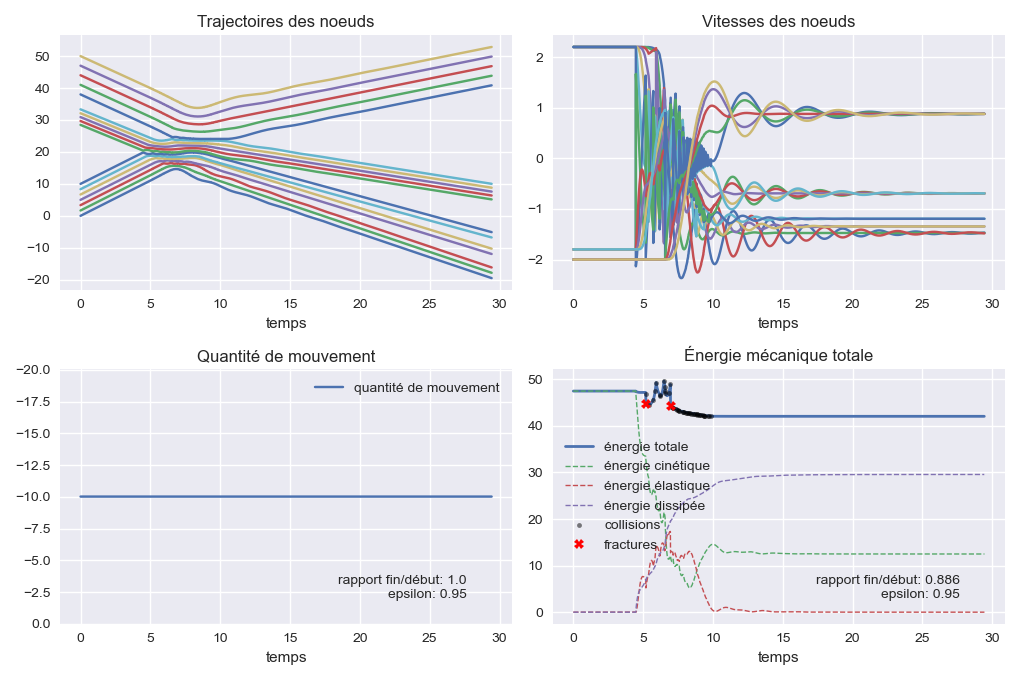
\includegraphics[width=.85\textwidth]{EnergieTotFrac.png}
    \caption{Étude de l'énergie mécanique totale du système. On observe une fluctuation intense de cette énergie, jusqu'à atteindre une valeur supérieure à l'énergie mécanique initiale. La simulation correspondante se trouve en pièce jointe.}
    \label{fig:energietot}
  \end{figure}
\end{enumerate} 





%----------------------------------------------------------------------------------------
% ASSIGNMENT CONTENT - SECTION 3
% ----------------------------------------------------------------------------------------
\section*{Travail à venir}


Hormis la recherche de la raison pour laquelle l'énergie mécanique ne diminue pas continuellement (ceci ne se produit que lorsqu'il y a fracture), la seule tache restante est la rédaction du rapport de stage.



% %-------------------------------------------------------------------------------
% %             THE BIBLIOGRAPHY
% %-------------------------------------------------------------------------------
\clearpage   % Pour retirer les references de la bare de navigation
\printbibliography


\end{document}
